\documentclass{article}

\usepackage{alltt}
\usepackage{amsmath}
\usepackage{amssymb}
\usepackage{amsthm}
\usepackage{array}
\usepackage[T1]{fontenc}
\usepackage{geometry}
\usepackage{graphicx}
\usepackage{multicol}
\usepackage{semantic}
\usepackage{tabularx}

\theoremstyle{definition}
\newtheorem{theorem}{Theorem}
\newtheorem{corollary}{Corollary}
\newtheorem{lemma}{Lemma}
\newtheorem{definition}{Definition}

\newcommand{\at}{\ensuremath{{\scriptstyle{@}}}}
\newcommand{\pc}{\ensuremath{{\mathit{pc}}}}

\newcommand{\CoqSymbol}
{\raisebox{-.2ex}{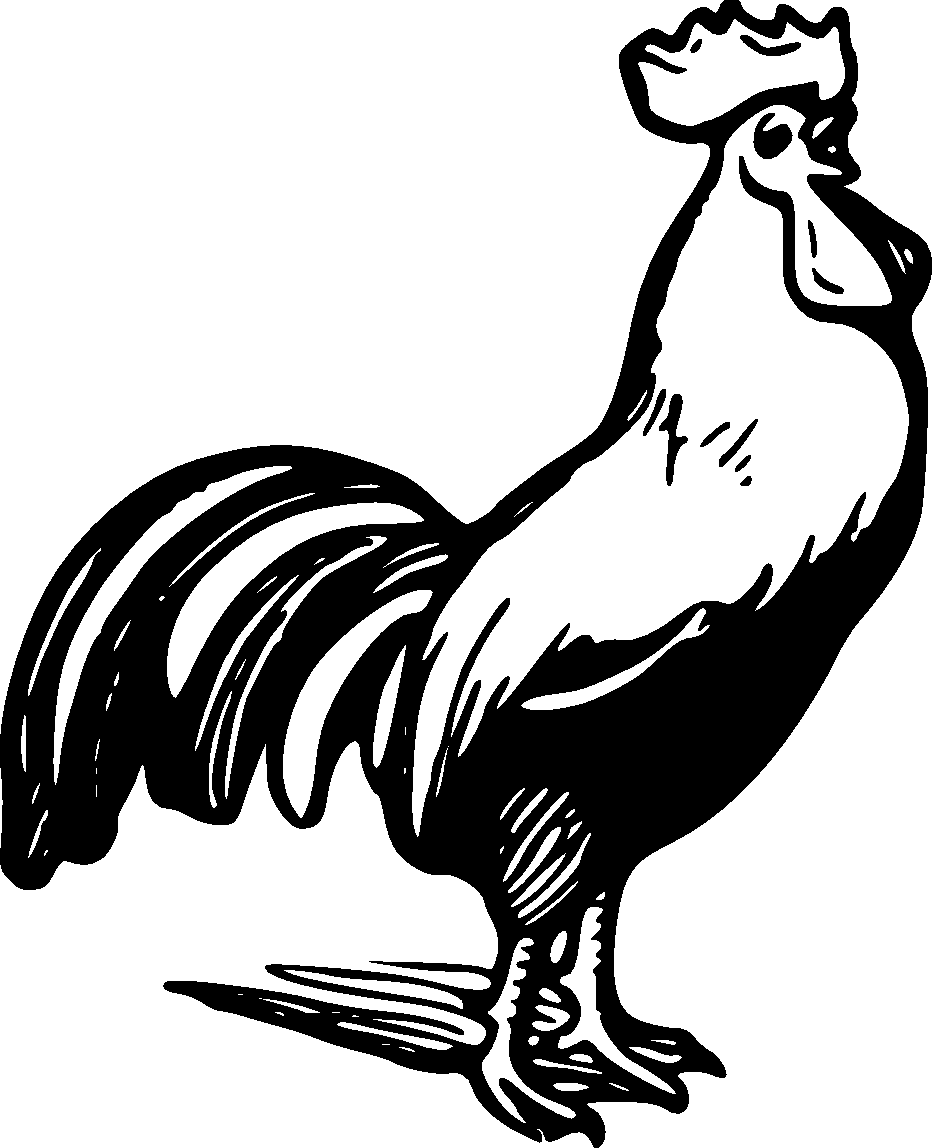
\includegraphics[height=0.9em]{coq.pdf}}\,}
\newcommand{\Coqed}{\hfill\CoqSymbol}

\renewcommand*{\descriptionlabel}[1]{\hspace\labelsep\normalfont #1}

\begin{document}

\begin{flushright}
  \today
\end{flushright}
%\begin{center}
%  {\Large{Multiple Security Levels}}
%\end{center}

\paragraph{Multiple Security Levels}
Let $\mathcal{M}_{0}$ be the 0-authority projection of any label algebra
$\mathcal{M}$.

\begin{figure}[ht]
  \centering
  \[
  \begin{array}[t]{lcl}
    b & ::= &
    \mathit{tt}\;\; |\;\;
    \mathit{ff}
    \\[0.3ex]
    c & :: = &
    b\;\; |\;\;
    n
    \\[0.3ex]
    e & ::= &
    c\;\; |\;\;
    x\;\; |\;\;
    \lambda{x}.\, e\;\; |\;\;
    e\ e\;\; |\;\;
    e \updownarrow L\;\; |\;\;
    \mathsf{if}\ e\ \mathsf{then}\ e\ \mathsf{else}\ e
    \\[0.3ex]
    v & ::= &
    c\;\; |\;\;
    \langle{\lambda{x}.\, e, \rho\rangle}
    \\[0.3ex]
    a & ::= &
    v \at L
    \\[0.3ex]
    \rho & ::= &
    \bullet\;\; |\;\;
    \rho[x = a]
  \end{array}
  \]
  \caption{Syntax of $\lambda_{\mathcal{M}_{0}}$.}
  \label{fig:syntax}
\end{figure}

\begin{definition}
  We say that labels $L_1$ and $L_2$ are \emph{indistinguishable at
    level $L$}, written $L_1 \approx^{L} L_2$, iff
  \begin{itemize}
  \item
    $L_1 \not\sqsubseteq L$ and
    $L_2 \not\sqsubseteq L$; or
  \item
    $L_1 \sqsubseteq L$ and
    $L_1 \equiv L_2$.
  \end{itemize}
  \label{def:lab-equiv}
\end{definition}

\begin{definition}
  Let $P$ be an equivalence relation on values. We say that atoms
  $v_1 \at L_1$ and $v_2 \at L_2$ are \emph{indistinguishable mod $P$ at
    level $L$}, written $v_1 \at L_1 \approx^{L}_{P} v_2 \at L_2$, iff
  \begin{itemize}
  \item
    $L_1 \not\sqsubseteq L$ and
    $L_2 \not\sqsubseteq L$ and
    \begin{itemize}
    \item
      $v_1 = n_1$ and
      $v_2 = n_2$ and
      $P(v_1, v_2)$, or
    \item
      $v_1 = \langle{\lambda{x_1}.\, e_1, \rho_1\rangle}$ and
      $v_2 = \langle{\lambda{x_2}.\, e_2, \rho_2\rangle}$ and
      $v_1 \approx^{L}_{P} v_2$, or
    \item
      $v_1 = c_1$ and $v_2 = \langle{\lambda{x_2}.\, e_2, \rho_2\rangle}$, or
    \item
      $v_1 = \langle{\lambda{x_1}.\, e_1, \rho_1\rangle}$ and $v_2 = c_2$; or
    \end{itemize}
  \item
    $L_1 \sqsubseteq L$ and $L_1 \equiv L_2$ and $v_1 \approx^{L}_{P} v_2$.
  \end{itemize}
  The definition for atoms is mutually recursive with that for values and
  environments:
  \begin{itemize}
  \item $c_1 \approx^{L}_{P} c_2$ iff $c_1 = c_2$.
  \item
    $\langle{\lambda{x_1}.\, e_1, \rho_1\rangle} \approx^{L}_{P}
    \langle{\lambda{x_2}.\, e_2, \rho_2\rangle}$ iff
    $\lambda{x_1}.\, e_1 \equiv \lambda{x_2}.\, e_2$ and
    $\rho_1 \approx^{L}_{P} \rho_2$.
  \item $\rho_1 \approx^{L}_{P} \rho_2$ iff
    $\mathrm{dom}\; \rho_1 = \mathrm{dom}\; \rho_2$ and
    $\rho_1(x) \approx^{L}_{P} \rho_2(x)$ for every
    $x \in \mathrm{dom}\; \rho_1$.
  \end{itemize}
  \label{def:atom-equiv}
\end{definition}

\begin{lemma}
  $\approx^{L}$ is reflexive, symmetric, and transitive.
  \Coqed
  \label{lem:lab-equiv-rst}
\end{lemma}
\begin{lemma}
  $\approx^{L}_{P}$ is reflexive and symmetric.
  \Coqed
  \label{lem:atom-equiv-rs}
\end{lemma}
\begin{lemma}
  If $v_1 \at L_1 \approx^{L}_{P} v_2 \at L_2$ and
  $L_1' \approx^{L} L_2'$, then
  $v_1 \at (L_1 \sqcup L_1') \approx^{L}_{P} v_2 \at (L_2 \sqcup L_2')$.
  \Coqed
  \label{lem:atom-equiv-raise}
\end{lemma}

\pagebreak

\begin{figure}[ht]
  \centering
  \begin{gather*}
    \inference{}{
      \pc, \rho |-
      c
      \Downarrow^{k}_{m}
      c \at \pc
    }[\textsc{E-Const}]
    \qquad
    \inference{
      {\begin{array}{l}
          \rho(x) = v \at L_1
        \end{array}}
    }{
      \pc, \rho |-
      x
      \Downarrow^{k}_{m}
      v \at (\pc \sqcup L_1)
    }[\textsc{E-Var}]
    \\[3ex]
    \inference{}{
      \pc, \rho |-
      (\lambda{x}.\, e)
      \Downarrow^{k}_{m}
      \langle{\lambda{x}.\, e, \rho\rangle} \at \pc
    }[\textsc{E-Abs}]
    \\[3ex]
    \inference{
      \pc, \rho |-
      e_1
      \Downarrow^{k}_{m}
      \langle{\lambda{x}.\, e, \rho_1\rangle} \at L_1
      \\
      \pc, \rho |-
      e_2 \Downarrow^{k}_{m} a_2
      &
      L_1, \rho_1[x = a_2] |-
      e
      \Downarrow^{k}_{m}
      a_3
    }{
      \pc, \rho |-
      (e_1\ e_2)
      \Downarrow^{k+1}_{m}
      a_3
    }[\textsc{E-App}]
    \\[3ex]
    \inference{
      \pc, \rho |-
      e
      \Downarrow^{k}_{m}
      v \at L_1
      &
      L_1 \sqsubseteq L_2
    }{
      \pc, \rho |-
      e \updownarrow L_2
      \Downarrow^{k+1}_{m}
      v \at L_2
    }[\textsc{E-Relabel1}]
    \\[3ex]
    \inference{
      \pc, \rho |-
      e
      \Downarrow^{k}_{m}
      v \at L_1
      &
      L_2 \sqsubseteq L_1
      \\
      \forall{\pc' \approx^{L} \pc,
        \rho' \approx^{L}_{P} \rho,
        L_1' \approx^{L} L_1}.
      \qquad\\\quad
      \pc', \rho' |-
      e
      \Downarrow^{m}_{k}
      v' \at L_1'
      ==>
      v \approx^{L}_{P} v'
    }{
      \pc, \rho |-
      e \updownarrow L_2
      \Downarrow^{k+1}_{m}
      v \at L_2
    }[\textsc{E-Relabel2}]
    \\[3ex]
    \inference{
      \pc, \rho |- e_1 \Downarrow^{k}_{m} \mathit{tt} \at L_1
      &
      L_1 \sqsubseteq L
      \\
      (\pc \sqcup L_1), \rho |- e_2 \Downarrow^{k}_{m} a_2
    }{
      \pc, \rho |-
      \mathsf{if}\ e_1\ \mathsf{then}\ e_2\ \mathsf{else}\ e_3
      \Downarrow^{k+1}_{m}
      a_2
    }[\textsc{E-IfTrue}]
    \\[3ex]
    \inference{
      \pc, \rho |- e_1 \Downarrow^{k}_{m} \mathit{ff} \at L_1
      &
      L_1 \sqsubseteq L
      \\
      (\pc \sqcup L_1), \rho |- e_3 \Downarrow^{k}_{m} a_3
    }{
      \pc, \rho |-
      \mathsf{if}\ e_1\ \mathsf{then}\ e_2\ \mathsf{else}\ e_3
      \Downarrow^{k+1}_{m}
      a_3
    }[\textsc{E-IfFalse}]
  \end{gather*}
  \caption{Semantics of $\lambda_{\mathcal{M}_{0}}$.}
  \label{fig:semantics}
\end{figure}

\begin{definition}
  $\pc, \rho |- e \Downarrow a\, <=>\,
  \exists{k}.\, \forall{m}.\, \pc, \rho |- e \Downarrow^{k}_{m} a$
  \label{def:eval}
\end{definition}

\begin{lemma}
  $\Downarrow^{k}_{m}\ \subseteq\ \Downarrow^{k+1}_{m}$
  and
  $\Downarrow^{k}_{m+1}\ \subseteq\ \Downarrow^{k}_{m}$.
  \Coqed
  % \begin{enumerate}
  % \item
  %   If $\pc, \rho |- e \Downarrow^{k}_{m} a$, then
  %   $\pc, \rho |- \Downarrow^{k+1}_{m} a$.
  % \item
  %   If $\pc, \rho |- e \Downarrow^{k}_{m+1} a$, then
  %   $\pc, \rho |- e \Downarrow^{k}_{m} a$.
  %   \Coqed
  % \end{enumerate}
  \label{lem:semantics-mon}
\end{lemma}

\begin{theorem}
  For any observer labeled $L$, if
  \begin{itemize}
  \item
    $\pc_1, \rho_1 |- e \Downarrow a_1$,
  \item
    $\pc_2, \rho_2 |- e \Downarrow a_2$,
  \item
    $\pc_1 \approx^{L} \pc_2$, and
  \item
    $\rho_1 \approx^{L}_{P} \rho_2$,
  \end{itemize}
  then $a_1 \approx^{L}_{P} a_2$.
  \Coqed
  \label{thm:non-interference}
\end{theorem}

\end{document}
